\subsection{Communication entre composants}

% \subsubsection{Problématique et logique de communication}

La programmation des protocoles de communications entre les différents composants
électroniques dans un système temps réel se révèle être un éléments clé pour le bon
fonctionnement de ce dernier mais aussi ardu à mettre en place. Il n'est par exemple
pas souhaitable de bloquer certaines tâches du système lors de la transmission ou
de la réception de données entre les composants. C'est notamment pour cela que le
choix d'un microcontrôleur contre un microprocesseur a été fait. En effet, un
microcontrôleur est capable de gérer des interruptions matérielles bien plus
facilement et efficacement qu'un microprocesseur seul grâce aux périphériques
intégrés de ce premier. Néanmoins une vigilent plus importante comparé à un
système séquentiel est nécessaire. En effet, il est possible de se retrouver avec
des problèmes de synchronisation entre les différents composants électroniques. Il
faut ainsi être capable de ne pas permettre à deux tâches d'intéragir avec des
composants utilisant le même bus de communication en même temps.\\

\subsubsection{Présentation du concepte}

Prenons l'exemple d'une communication SPI. Il est possible de partager un bus SPI
entre plusieurs composants électroniques. Cependant, il est nécessaire de s'assurer
que le bus SPI soit bien libre avant de pouvoir transmettre ou recevoir des données.
Voici l'implémentation de quelques outils permettant de gérer la communication SPI
de manière asynchrone.

\begin{lstlisting}[style=prog, frame=shadowbox, caption={Définition des outlis spi suplémentaires (tools.h)}, label={lst:tools_h},
    emph={[1]SPI_HandleTypeDef_flag_init, ASYNC_SPI_TxRx_DMA_init, ASYNC_SPI_TxRx_DMA, add_task, kill_task, run_task,
    run_scheduler}, emphstyle={[1]\color{C}},
    emph={[2]GPIO_TypeDef, SCHEDULER, TASK, SPI_HandleTypeDef, SPI_HandleTypeDef_flag, ASYNC_DMA_STATE, ASYNC_SPI_TxRx_DMA_CONTEXT}, emphstyle={[2]\color{E}}]
#include <string.h>

typedef struct SPI_HandleTypeDef_flag {
    SPI_HandleTypeDef *hspi;
    bool               is_used;
} SPI_HandleTypeDef_flag;

typedef struct ASYNC_SPI_TxRx_DMA_CONTEXT {
    SPI_HandleTypeDef_flag *hspi_flag;
    GPIO_TypeDef           *csPinBank;
    uint16_t                csPin;
    bool                    has_started;
    uint8_t                *tx_buf;
    uint8_t                *rx_buf;
    uint16_t                tx_size;
    uint16_t                rx_size;
} ASYNC_SPI_TxRx_DMA_CONTEXT;

// Initialise la structure SPI\_HandleTypeDef\_flag
void SPI_HandleTypeDef_flag_init(SPI_HandleTypeDef_flag *hspi_flag,
                                 SPI_HandleTypeDef* hspi);

// Initialise le contexte de la tâche ASYNC\_SPI\_TxRx\_DMA
void ASYNC_SPI_TxRx_DMA_init(...);

// Tâche permettant de transmettre et recevoir des données en SPI en asynchrone
void ASYNC_SPI_TxRx_DMA(SCHEDULER* scheduler, TASK* self);
\end{lstlisting}

\newpage

\begin{lstlisting}[style=prog, frame=shadowbox, caption={Implémentation des outlis spi suplémentaires (tools.c)}, label={lst:tools_c},
    emph={[1]malloc, free, memcpy, SPI_HandleTypeDef_flag_init, ASYNC_SPI_TxRx_DMA_init, ASYNC_SPI_TxRx_DMA, add_task, kill_task, run_task,
    run_scheduler, HAL_GPIO_WritePin, HAL_SPI_TransmitReceive_DMA, HAL_SPI_STATE_READY, GPIO_PIN_SET, GPIO_PIN_RESET}, emphstyle={[1]\color{C}},
    emph={[2]GPIO_TypeDef, SCHEDULER, TASK, SPI_HandleTypeDef, SPI_HandleTypeDef_flag, ASYNC_DMA_STATE, ASYNC_SPI_TxRx_DMA_CONTEXT}, emphstyle={[2]\color{E}}]
void SPI_HandleTypeDef_flag_init(SPI_HandleTypeDef_flag *hspi_flag,
                                 SPI_HandleTypeDef      *hspi) {
    hspi_flag->hspi = hspi;
    hspi_flag->is_used = false;
}

void ASYNC_SPI_TxRx_DMA_init(TASK                       *task,
                             SPI_HandleTypeDef_flag     *hspi_flag,
                             GPIO_TypeDef               *csPinBank,
                             uint16_t                    csPin,
                             uint8_t                    *tx_buf,
                             uint8_t                    *rx_buf,
                             uint16_t                    tx_size,
                             uint16_t                    rx_size) {
    ASYNC_SPI_TxRx_DMA_CONTEXT *context=(ASYNC_SPI_TxRx_DMA_CONTEXT*)task->context;

    context->hspi_flag = hspi_flag;
    context->csPinBank = csPinBank;
    context->csPin = csPin;

    context->owner_task = owner_task;

    context->has_started = false;

    context->tx_buf = tx_buf;
    context->rx_buf = rx_buf;
    context->tx_size = tx_size;
    context->rx_size = rx_size;

    uint16_t size = tx_size + rx_size;

    context->__tx_buf_full = (uint8_t*)malloc(sizeof(uint8_t) * size);
    context->__rx_buf_full = (uint8_t*)malloc(sizeof(uint8_t) * size);

    memcpy(context->__tx_buf_full,
           context->tx_buf,
           context->tx_size);
}

void ASYNC_SPI_TxRx_DMA(SCHEDULER *scheduler, TASK *self) {
    ASYNC_SPI_TxRx_DMA_CONTEXT* context=(ASYNC_SPI_TxRx_DMA_CONTEXT*)self->context;

    uint16_t size = context->tx_size + context->rx_size;

    if (context->hspi_flag->hspi->State == HAL_SPI_STATE_READY) {
        if ((!context->has_started) && (!context->hspi_flag->is_used)) {
            context->has_started = true;
            context->hspi_flag->is_used = true;     // Prend le controle du bus SPI
            HAL_GPIO_WritePin(context->csPinBank, context->csPin, GPIO_PIN_RESET);
            HAL_SPI_TransmitReceive_DMA(context->hspi_flag->hspi,
                                        context->__tx_buf_full,
                                        context->__rx_buf_full,
                                        size);
        } else if ((context->has_started) && (context->hspi_flag->is_used)) {
            HAL_GPIO_WritePin(context->csPinBank, context->csPin, GPIO_PIN_SET);
            context->hspi_flag->is_used = false;    // Realease SPI bus
            if (context->rx_buf) {                  // rx\_buf peut être NULL
                memcpy(context->rx_buf,
                       context->__rx_buf_full + context->tx_size,
                       context->rx_size);
            }
            free(context->__tx_buf_full);
            free(context->__rx_buf_full);
            kill_task(scheduler, self);
        }
    }
}

\end{lstlisting}

Bien que la couche d'abstraction matérielle (HAL) du microcontrôleur STM32 propose
le type de structure \texttt{SPI\_HandleTypeDef} pour gérer les bus SPI, il a été
jugé plus pertinent de créer une structure supplémentaire
\texttt{SPI\_HandleTypeDef\_flag} notamment pour gérer l'état du bus SPI. En effet,
bien qu'un \texttt{SPI\_HandleTypeDef} ait un attribut \texttt{State} permettant de
connaître l'état du bus SPI et donc de savoir s'il est prêt à être utilisé, il est
possible de se retrouver dans une situation où une tâche B souhaite utiliser le bus
SPI alors qu'une tâche A n'ait pas fini de cloturer complètement son utilisation du
bus SPI, en changeant notamment l'état du pin \texttt{CS} (Chip Select).

Aussi, la fonction \texttt{HAL\_SPI\_TransmitReceive\_DMA}, servant à démarrer une
transmission et réception de données en SPI en asynchrone, a un comportement qui
permet d'envoyer et de recevoir des données en même temps. Cependant, le
comportement souhaité dans la majeur partie des composants électroniques est de
transmettre puis de recevoir des données. Il a été donc été décidé d'ajouter des
buffers supplémentaires \texttt{\_\_tx\_buf\_full} et \texttt{\_\_rx\_buf\_full}
afin de simuler un comportement plus attendu de la fonction.\\

\begin{figure}[h]
    \centering
    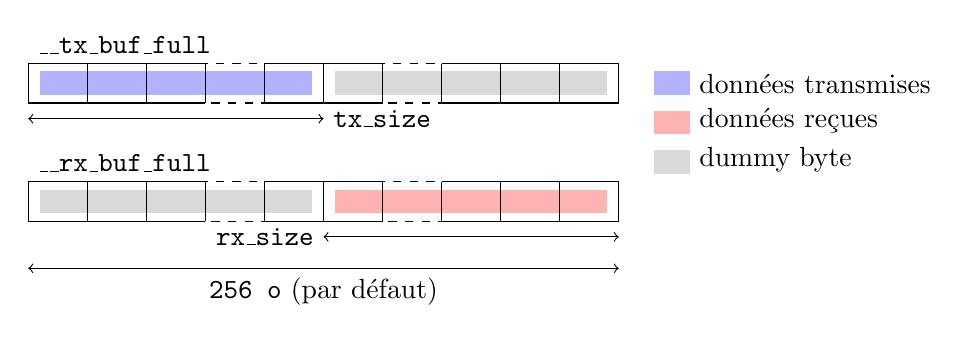
\begin{tikzpicture}[yscale=1, xscale=1.5]
        % \draw[help lines] (0, 0) grid (10, 5);

        \draw node at   (0.0, 2.0) [anchor=south west] {\texttt{\_\_tx\_buf\_full}};
        \fill[blue!30]  (0.1, 1.6) rectangle (2.4, 1.9);
        \fill[gray!30]  (2.6, 1.6) rectangle (4.9, 1.9);
        \draw[step=0.5] (0.0, 1.5) grid      (1.5, 2.0);
        \draw[dashed]   (1.5, 1.5) rectangle (2.0, 2.0);
        \draw[step=0.5] (2.0, 1.5) grid      (3.0, 2.0);
        \draw[dashed]   (3.0, 1.5) rectangle (3.5, 2.0);
        \draw[step=0.5] (3.5, 1.5) grid      (5.0, 2.0);
        \draw           (2.0, 1.5) --        (2.0, 2.0);
        \draw           (3.5, 1.5) --        (3.5, 2.0);
        \draw           (0.0, 1.5) --        (1.5, 1.5);
        \draw           (2.0, 1.5) --        (3.0, 1.5);
        \draw           (3.5, 1.5) --        (5.0, 1.5);
        \draw[<->]      (0.0, 1.3) --        (2.5, 1.3) node[right] {\texttt{tx\_size}};

        
        \draw node at   (0.0,  0.5) [anchor=south west] {\texttt{\_\_rx\_buf\_full}};
        \fill[gray!30]  (0.1,  0.1) rectangle (2.4,  0.4);
        \fill[red!30]   (2.6,  0.1) rectangle (4.9,  0.4);
        \draw[step=0.5] (0.0,  0.0) grid      (1.5,  0.5);
        \draw[dashed]   (1.5,  0.0) rectangle (2.0,  0.5);
        \draw[step=0.5] (2.0,  0.0) grid      (3.0,  0.5);
        \draw[dashed]   (3.0,  0.0) rectangle (3.5,  0.5);
        \draw[step=0.5] (3.5,  0.0) grid      (5.0,  0.5);
        \draw           (2.0,  0.0) --        (2.0,  0.5);
        \draw           (3.5,  0.0) --        (3.5,  0.5);
        \draw           (0.0,  0.0) --        (1.5,  0.0);
        \draw           (2.0,  0.0) --        (3.0,  0.0);
        \draw           (3.5,  0.0) --        (5.0,  0.0);
        \draw[<->]      (2.5, -0.2) node[left]{\texttt{rx\_size}} -- (5.0, -0.2);
    
        \draw[<->]      (0.0, -0.6)  -- (5.0, -0.6) node[midway, below]{\texttt{256 o} (par défaut)};

        \fill[blue!30]  (5.3, 1.6) rectangle (5.6, 1.9);
        \draw node at   (5.6, 1.5) [anchor=south west] {données transmises};
        \fill[red!30]   (5.3, 1.1) rectangle (5.6, 1.4);
        \draw node at   (5.6, 1.0) [anchor=south west] {données reçues};
        \fill[gray!30]  (5.3, 0.6) rectangle (5.6, 0.9);
        \draw node at   (5.6, 0.5) [anchor=south west] {dummy byte};
    \end{tikzpicture}
    \caption{Représentation des buffers \texttt{\_\_tx\_buf\_full} et \texttt{\_\_rx\_buf\_full}}
    \label{fig:async_spi_buffers}
\end{figure}

Pour résumer la routine d'une communication SPI en asynchrone : une fois que la
tâche est ajoutée au \texttt{scheduler} et que son context est initialisé, elle
attend que le bus SPI soit prêt à être utilisé. Une fois que le périphérique SPI
est prêt, trois cas de figure peuvent se présenter:
\begin{itemize}
    \item \textbf{La tâche n'a pas encore démarrer une communication SPI et le bus
    est libre.}\newline     La tâche peut donc prendre le contrôle du bus SPI et
    initier une communication SPI en activant le pin \texttt{CS} donné en paramètre
    et en appelant la fonction \texttt{HAL\_SPI\_TransmitReceive\_DMA}.
    \item \textbf{La tâche n'a pas encore démarrer une communication SPI mais le
    bus n'est pas libéré.}\newline Cela signifie qu'une autre tâche avait déjà
    entamé une communication SPI et cette dernière n'a pas cloturer complètement
    son utilisation du bus SPI et un pin \texttt{CS} est actif. La tâche doit donc
    attendre que le bus SPI soit libéré.
    \item \textbf{La tâche a déjà démarré une communication SPI et le bus SPI est
    occupé.}\newline Dans ce cas, la tâche qui avait déjà entamé une communication
    SPI est la tâche en cours. Elle peut donc cloturer sa communication SPI en
    désactivant le pin \texttt{CS}, en copiant les données reçues du buffer
    \texttt{\_\_rx\_buf\_full} vers le buffer \texttt{rx\_buf} (sans prendre en
    compte les dummy bit) et en libérant le bus SPI. La tâche peut alors se terminer.\\
\end{itemize}

\newpage

Avec ce fonctionnement, tous processuces peut appeler plusieurs tâches
\texttt{ASYNC\_SPI\_TxRx\_DMA} simultanément et les requêtes seront traitées
séquentiellement sans qu'il n'y ait de problème de synchronisation et sans bloquer
le système. Une tâche voulant utiliser le bus SPI sera la plupart du temps
construite comme une machine à 3 états dont les états sont définies par
l'\texttt{enum} \texttt{ASYNC\_DMA\_STATE} :
\begin{itemize}
    \item \texttt{ASYNC\_DMA\_START} : la tâche n'a pas encore démarré une
    communication SPI et appelle la sous-tâche \texttt{ASYNC\_SPI\_TxRx\_DMA}.
    \item \texttt{ASYNC\_DMA\_WAIT} : la tâche a démarré une communication SPI et
    attend que la sous-tâche précédament appelée ait terminé complètement son
    exécution (utilisation de la fonction \texttt{kill\_task(...)} qui met à jour
    un drapeau partagé avec la tâche).
    \item \texttt{ASYNC\_DMA\_END} : la tâche a démarré une communication SPI et
    la sous-tâche précédament appelée a terminé son exécution. La tâche peut alors
    continuer son exécution en traitant notamment les données reçues si elle en
    attendait.    
\end{itemize}

Le même principe peut être appliqué pour d'autres protocoles de communication
comme l'I2C ou l'UART.

\subsubsection{Les tâches de communications}

Chaques tâches de communication se construisent sur le même modèle.

\begin{lstlisting}[style=prog, frame=shadowbox, caption={Patron d'une tâche de communication}, label={lst:async_pattern_comm},
    emph={[1]ASYNC____TxRx_DMA_init, ASYNC____TxRx_DMA}, emphstyle={[1]\color{C}},
    emph={[2]SCHEDULER, TASK, ASYNC_DMA_STATE, ASYNC_SPI_TxRx_DMA_CONTEXT}, emphstyle={[2]\color{E}}]
void ASYNC____TxRx_DMA_init(TASK     *task,
                            ...,
                            uint8_t  *tx_buf,
                            uint8_t  *rx_buf,
                            uint16_t  tx_size,
                            uint16_t  rx_size);

void ASYNC____TxRx_DMA(SCHEDULER *scheduler, TASK *self);
\end{lstlisting}

Elles prennent alors toutes en paramètre un tableau de données à transmettre
\texttt{tx\_buf}, un tableau de données à recevoir \texttt{rx\_buf}, la taille de ces
tableaux \texttt{tx\_size} et \texttt{rx\_size}. Si il n'est question que de
transmettre ou que de recevoir des données, il est possible de mettre \texttt{NULL}
pour le tableau de données. Cependant, il est nécessaire de préciser la taille du
tableau à 0. A noter que le tableau \texttt{tx\_buf} est copié dans un buffer interne
lors de l'appel de la fonction \texttt{ASYNC\_\_\_\_TxRx\_DMA\_init}. Il n'est donc
pas nécessaire de conserver le tableau \texttt{tx\_buf}.

La tâche se termine une fois que la communication SPI est terminée et que les données
reçues ont été copiées dans le tableau \texttt{rx\_buf}. Après la détection de la fin
de la tâche il est possible de traiter les données reçues présentent dans le tableau
\texttt{rx\_buf}.
